%%%%%%%%%%%%%%%%%%%%%%%%%%%%%%%%%%%%%%%%%
% Journal Article
% LaTeX Template
% Version 1.4 (15/5/16)
%
% This template has been downloaded from:
% http://www.LaTeXTemplates.com
%
% Original author:
% Frits Wenneker (http://www.howtotex.com) with extensive modifications by
% Vel (vel@LaTeXTemplates.com)
%
% License:
% CC BY-NC-SA 3.0 (http://creativecommons.org/licenses/by-nc-sa/3.0/)
%
%%%%%%%%%%%%%%%%%%%%%%%%%%%%%%%%%%%%%%%%%

%----------------------------------------------------------------------------------------
%	PACKAGES AND OTHER DOCUMENT CONFIGURATIONS
%----------------------------------------------------------------------------------------

\documentclass[twoside,onecolumn]{article}

\usepackage{blindtext} % Package to generate dummy text throughout this template 

% \usepackage[sc]{mathpazo} % Use the Palatino font
% \usepackage[T1]{fontenc} % Use 8-bit encoding that has 256 glyphs
\usepackage{fontspec}
\setmainfont{TeX Gyre Pagella}
\usepackage{unicode-math}
\setmathfont{Latin Modern Math}
\linespread{1.05} % Line spacing - Palatino needs more space between lines
\usepackage{microtype} % Slightly tweak font spacing for aesthetics

\usepackage[english]{babel} % Language hyphenation and typographical rules

\usepackage[hmarginratio=1:1,top=32mm,columnsep=20pt]{geometry} % Document margins
\usepackage[hang, small,labelfont=bf,up,textfont=it,up]{caption} % Custom captions under/above floats in tables or figures
\usepackage{booktabs} % Horizontal rules in tables

\usepackage{lettrine} % The lettrine is the first enlarged letter at the beginning of the text

\usepackage{enumitem} % Customized lists
\setlist[itemize]{noitemsep} % Make itemize lists more compact

\usepackage{abstract} % Allows abstract customization
\renewcommand{\abstractnamefont}{\normalfont\bfseries} % Set the "Abstract" text to bold
\renewcommand{\abstracttextfont}{\normalfont\small\itshape} % Set the abstract itself to small italic text

\usepackage{titlesec} % Allows customization of titles
\renewcommand\thesection{\Roman{section}} % Roman numerals for the sections
\renewcommand\thesubsection{\roman{subsection}} % roman numerals for subsections
\titleformat{\section}[block]{\large\scshape\centering}{\thesection.}{1em}{} % Change the look of the section titles
\titleformat{\subsection}[block]{\large}{\thesubsection.}{1em}{} % Change the look of the section titles

\usepackage{fancyhdr} % Headers and footers
\pagestyle{fancy} % All pages have headers and footers
\fancyhead{} % Blank out the default header
\fancyfoot{} % Blank out the default footer
\fancyhead[C]{Journal MusMat $\bullet$ Month Year $\bullet$ Vol. X, No. X} % Custom header text
\fancyfoot[RO,LE]{\thepage} % Custom footer text

\usepackage{titling} % Customizing the title section

\usepackage{hyperref} % For hyperlinks in the PDF
% Colors for hyperlinks  ----------
\usepackage[dvipsnames]{xcolor}
\newcommand\myshade{85}
\definecolor{mycitecolor}{RGB}{197, 55, 19}
\definecolor{mylinkcolor}{RGB}{197, 55, 19}
\definecolor{myurlcolor}{RGB}{197, 55, 19}

\hypersetup{
  linkcolor  = mylinkcolor!\myshade!black,
  citecolor  = mycitecolor!\myshade!black,
  urlcolor   = myurlcolor!\myshade!black,
  colorlinks = true,
}
%----------------------------------
\usepackage{graphicx}
\usepackage{amsfonts}
\usepackage{amsmath}
\usepackage{subfig}
\usepackage{textcomp}
%----------------------------------------------------------------------------------------
%	TITLE SECTION
%----------------------------------------------------------------------------------------
\setlength{\droptitle}{-4\baselineskip} % Move the title up

\pretitle{\begin{center}\Huge\bfseries} % Article title formatting
\posttitle{\end{center}} % Article title closing formatting
%--------------- Article title
\title{Diatonicism vs Chromaticism: data-driven perspectives on style in music}

%--------------- Author informations
\author{
\thanks {I am grateful to Robert Lieck and Zeng Ren for valuable discussions.}
\textsc{Fabian C. Moss}\\ %Your name
\normalsize  {Julius-Maximilians-Universität Würzburg}\\
\ttfamily
\normalsize \href{mailto:fabian.moss@uni-wuerzburg.de}
{fabian.moss@uni-wuerzburg.de} \\% Your email address
\normalfont
% \\
% \textsc{Second Author}\\ % Co-autor's name
% \normalsize  {Institution}\\ 
% \ttfamily
% \normalsize \href{mailto:email@email.com}{email@email.com} \\
% \normalfont
}

%\and % Uncomment if 2 authors are required, duplicate these 4 lines if more
%\textsc{Jane Smith}\thanks{Corresponding author} \\[1ex] % Second author's name
%\normalsize University of Utah \\ % Second author's institution
%\normalsize \href{mailto:jane@smith.com}{jane@smith.com} % Second author's email address

\date{} % Leave empty to omit a date
\renewcommand{\maketitlehookd}{%
\renewcommand{\abstractname}{\vspace{-\baselineskip}}

%%%%%%% NOTES %%%%%%%%%%%
%%%%%%%%%%%%%%%%%%%%%%%%%

\begin{abstract}
\noindent \textbf{Abstract:} Lorem ipsum dolor sit amet, consectetuer adipiscing elit. Etiam lobortis facilisis sem. Nullam nec mi et neque pharetra sollicitudin. Praesent imperdiet mi nec ante. Donec ullamcorper, felis non sodales commodo, lectus velit ultrices augue, a dignissim nibh lectus placerat pede. Vivamus nunc nunc, molestie ut, ultricies vel, semper in, velit. Ut porttitor. Praesent in sapien. Lorem ipsum dolor sit amet, consectetuer adipiscing elit. Duis fringilla tristique neque. Sed interdum libero ut metus. Pellentesque placerat. Nam rutrum augue a leo. Morbi sed elit sit amet ante lobortis sollicitudin. Praesent blandit blandit mauris. Praesent lectus tellus, aliquet aliquam, luctus a, egestas a, turpis. Mauris lacinia lorem
sit amet ipsum. Nunc quis urna dictum turpis accumsan semper.\\

\noindent \textbf{Keywords}: 1--5 keywords.


\end{abstract}
}

%----------------------------------------------------------------------------------------

\begin{document}

% Print the title
\maketitle

%----------------------------------------------------------------------------------------
%	ARTICLE CONTENTS
%----------------------------------------------------------------------------------------

\section{Introduction}\label{sec:intro}

\lettrine[nindent=0em,lines=3] {L}orem ipsum dolor sit amet, consectetuer adipiscing elit (\cite[p. 34-39]{Figueredo:2009}. Etiam lobortis facilisis sem. Nullam nec mi et neque pharetra sollicitudin. Praesent imperdiet mi nec ante. Donec ullamcorper, felis non sodales commodo, lectus velit ultrices augue, a dignissim nibh lectus placerat pede. Vivamus nunc nunc, molestie ut, ultricies vel, semper in, velit. Ut porttitor. Praesent in sapien. Lorem ipsum dolor sit amet, consectetuer adipiscing elit. Duis fringilla tristique neque. Sed interdum libero ut metus. Pellentesque placerat. Nam rutrum augue a leo. Morbi sed elit sit amet ante lobortis sollicitudin. Praesent blandit blandit mauris. Praesent lectus tellus, aliquet aliquam, luctus a, egestas a, turpis. Mauris lacinia lorem
sit amet ipsum. Nunc quis urna dictum turpis accumsan semper..

\begin{quote}
Lorem ipsum dolor sit amet, consectetuer adipiscing elit (\cite[p. 34-39]{Figueredo:2009}. Etiam lobortis facilisis sem. Nullam nec mi et neque pharetra sollicitudin. Praesent imperdiet mi nec ante. Donec ullamcorper, felis non sodales commodo, lectus velit ultrices augue, a dignissim nibh lectus placerat pede. Vivamus nunc nunc, molestie ut, ultricies vel, semper in, velit. Ut porttitor. Praesent in sapien. Lorem ipsum dolor sit amet, consectetuer adipiscing elit. Duis fringilla tristique neque. Sed interdum libero ut metus. Pellentesque placerat. Nam rutrum augue a leo. Morbi sed elit sit amet ante lobortis sollicitudin. Praesent blandit blandit mauris. Praesent lectus tellus, aliquet aliquam, luctus a, egestas a, turpis. Mauris lacinia lorem
sit amet ipsum. Nunc quis urna dictum turpis accumsan semper (\cite[p. 2]{Berry:1976}).
\end{quote}

\blindtext % Dummy text

Text requiring further explanation\footnote{Example footnote}.

\section{Method}\label{sec:method}
\blindtext % Dummy text

\subsection{Data}\label{sec:data}

Use \textit{Enhanced Wikifonia Leadsheet Dataset}\footnote{\url{https://zenodo.org/record/1476555\#.ZP_9TdJBxhF}} (EWLD)? Compare with other historical corpora (e.g. Polish scores corpus, DCML data, CRIM). 

\blindtext % Dummy text

\begin{table}
\caption{Datasets used in the subsequent analyses.}
\centering
\begin{tabular}{llrr}
\toprule
% \multicolumn{2}{c}{Name} \\
% \cmidrule(r){1-2}
Name & Styles & Extent & Link \\
\midrule
Tonal Pitch-Class Counts Corpus (TP3C) & Western Classical & 1300--2000 & \cite{tp3c}\\
Classical Archives Corpus & Pop/Rock & & \\
Lakh MIDI & Pop &  & \\
Enhanced Wikifonia Leadsheet Dataset & Pop/Rock & & \\
\bottomrule
\label{tab1}
\end{tabular}
\end{table}

\subsection{Different scale orderings}\label{subsec22}

Fifth vs chromatic ordering. Well-formed scales

\blindtext % Dummy text


\subsection{DFT}

DFT-products \cite{YustAmiot:2022}

DFT matrix for 12 pitch classes

\textbf{Adapted from Wikipedia:}

An $N$-point DFT is expressed as the multiplication $X=Wx$, 
where $x$ is the original input signal, $W$ is the $N$-by-$N$ 
square DFT matrix, and $X$ is the DFT of the signal.

The transformation matrix $W$ can be defined as:

\begin{equation}
    W = \left({\frac {\omega ^{jk}}{\sqrt {N}}}\right)_{j,k=0,\ldots ,N-1}= \frac{1}{\sqrt{N}}{
    \begin{bmatrix}
        1&1&1&1&\cdots &1\\
        1&\omega &\omega ^{2}&\omega ^{3}&\cdots &\omega ^{N-1}\\
        1&\omega ^{2}&\omega ^{4}&\omega ^{6}&\cdots &\omega ^{2(N-1)}
        \\1&\omega ^{3}&\omega ^{6}&\omega ^{9}&\cdots &\omega ^{3(N-1)}\\
        \vdots &\vdots &\vdots &\vdots &\ddots &\vdots \\
        1&\omega ^{N-1}&\omega ^{2(N-1)}&\omega ^{3(N-1)}&\cdots &\omega ^{(N-1)(N-1)}
    \end{bmatrix}},    
\end{equation}


where $\omega =e^{-2\pi i/N}$ is a primitive $N$th root of unity in which $i^{2}=-1$. 
We can avoid writing large exponents for $\omega$ using the fact that for any exponent $x$ 
we have the identity 
\begin{equation}
    \omega^{x}=\omega^{x\mod N}.    
\end{equation}

This is the Vandermonde matrix for the roots of unity, up to the normalization factor. 
Note that the normalization factor in front of the sum ($1/{\sqrt {N}}$) 
and the sign of the exponent in $\omega$ are merely conventions, and differ in some treatments. 
All of the following discussion applies regardless of the convention, with at most minor adjustments. 
The only important thing is that the forward and inverse transforms have opposite-sign exponents,
and that the product of their normalization factors be $1/N$. However, the $1/\sqrt{N}$ choice here 
makes the resulting DFT matrix unitary, which is convenient in many circumstances.

Fast Fourier transform algorithms utilize the symmetries of the matrix to reduce the time
of multiplying a vector by this matrix, from the usual $O(N^{2})$. Similar techniques can be applied
for multiplications by matrices such as Hadamard matrix and the Walsh matrix.

\subsubsection{Pasted from ChatGPT: A Fourier-Theoretic Measure of Structural Preservation}

Let $P$ be a probability distribution over the twelve pitch classes, viewed as a function on the cyclic group

\[
\mathbb{Z}_{12} = \{0,\ldots,11\},
\]

with

\[
P(x)\ge0,\qquad
\sum_{x\in\mathbb Z_{12}}P(x)=1.
\]

Rather than viewing $P$ simply as a vector of probabilities, we regard it as a function on a finite Abelian group. This allows us to analyze its structure using harmonic analysis, where the natural basis is given by the irreducible characters of $\mathbb Z_{12}$.

The discrete Fourier transform (DFT) of $P$ is

\[
\widehat P(k)
=
\sum_{x=0}^{11}
P(x)
e^{-2\pi i kx/12},
\qquad
k=0,\ldots,11.
\]

The inverse transform is

\[
P(x)
=
\frac1{12}
\sum_{k=0}^{11}
\widehat P(k)
e^{2\pi i kx/12}.
\]

Thus the Fourier coefficients provide an alternative coordinate system for describing the pitch-class distribution.

\subsection{Interpretation of the Fourier coefficients}

Each Fourier coefficient corresponds to a periodic component of the pitch-class distribution.

The zeroth coefficient,

\[
\widehat P(0)=1,
\]

contains only the total probability mass.

The remaining coefficients describe cyclic periodicities.

For example,

\begin{center}
\begin{tabular}{cl}
$k$ & Approximate musical interpretation\\
\hline
1 & global orientation of the chromatic circle\\
2 & whole-tone polarity\\
3 & minor-third / diminished-seventh periodicity\\
4 & augmented-triad periodicity\\
6 & tritone polarity
\end{tabular}
\end{center}

Since $P$ is real-valued,

\[
\widehat P(12-k)
=
\overline{\widehat P(k)},
\]

so only six independent complex coefficients exist.

The magnitudes

\[
|\widehat P(k)|
\]

measure the strength of each periodicity, while the phases specify where that periodicity is located on the chromatic circle.

This decomposition is well established in computational music theory, where the Fourier coefficients are often interpreted as descriptors of intervallic structure.

\subsection{Automorphisms of the chromatic circle}

The multiplicative units of $\mathbb Z_{12}$ are

\[
\{1,5,7,11\},
\]

each defining an automorphism of the cyclic group.

Here we consider

\[
\pi(x)=7x\pmod{12}.
\]

Since

\[
7^2\equiv1\pmod{12},
\]

the map is an involution.

If

\[
Q(x)=P(\pi^{-1}(x)),
\]

then because $7^{-1}=7$,

\[
Q(x)=P(7x).
\]

This operation merely reorders the pitch classes.

Importantly, Shannon entropy, Kullback--Leibler divergence, and Jensen--Shannon divergence cannot distinguish $P$ from $Q$, since they depend only on the multiset of probabilities rather than on their assignment to pitch classes.

The Fourier transform, however, reveals how the automorphism acts on musical structure.

\subsection{Action on the Fourier spectrum}

The Fourier transform of $Q$ is

\[
\widehat Q(k)
=
\sum_x
Q(x)
e^{-2\pi i kx/12}.
\]

Substituting $Q(x)=P(7x)$ and changing variables gives

\[
\widehat Q(k)
=
\widehat P(7k\bmod12).
\]

Thus the automorphism does not distort the Fourier coefficients.

Instead, it permutes them.

The induced permutation is

\[
\begin{array}{c|cccccccccccc}
k      &0&1&2&3&4&5&6&7&8&9&10&11\\
\hline
7k\bmod12
       &0&7&2&9&4&11&6&1&8&3&10&5.
\end{array}
\]

Hence

\[
\begin{aligned}
0&\leftrightarrow0,\\
2&\leftrightarrow2,\\
4&\leftrightarrow4,\\
6&\leftrightarrow6,\\
8&\leftrightarrow8,\\
10&\leftrightarrow10,
\end{aligned}
\]

while

\[
(1\,7),\qquad
(3\,9),\qquad
(5\,11)
\]

are exchanged.

Consequently, all even Fourier modes are invariant under multiplication by seven, whereas the odd modes are reflected.

This decomposition provides a natural distinction between structural features that are preserved by the automorphism and those that are transformed.

\subsection{Spectral energy}

By Parseval's identity,

\[
\sum_{x=0}^{11}|P(x)|^2
=
\frac1{12}
\sum_{k=0}^{11}
|\widehat P(k)|^2.
\]

The quantities

\[
|\widehat P(k)|^2
\]

may therefore be interpreted as the distribution of structural energy across Fourier modes.

Normalizing gives

\[
E_k
=
\frac{
|\widehat P(k)|^2
}{
\sum_{j=0}^{11}
|\widehat P(j)|^2
},
\]

which satisfies

\[
E_k\ge0,
\qquad
\sum_kE_k=1.
\]

Thus $\{E_k\}$ forms a probability distribution over harmonic components rather than over pitch classes.

\subsection{Information retained by the automorphism}

Because multiplication by seven leaves the even Fourier modes fixed, a natural measure of structural preservation is the proportion of spectral energy contained within those invariant modes,

\[
R
=
\frac{
\sum_{k\in\{0,2,4,6,8,10\}}
|\widehat P(k)|^2
}{
\sum_{k=0}^{11}
|\widehat P(k)|^2
}.
\]

The quantity $R$ lies between $0$ and $1$.

Values near one indicate that most of the harmonic structure resides in Fourier modes that are invariant under the automorphism, implying that multiplication by seven preserves most of the distribution's structural organization.

Conversely, values near zero indicate that the structure depends primarily on odd Fourier modes, which are exchanged by the automorphism.

A more refined measure compares the entire spectra before and after transformation,

\[
C
=
\sum_{k=0}^{11}
w_k
\,
\widehat P(k)
\overline{\widehat P(7k)},
\]

where $w_k$ are non-negative weights reflecting the relative importance of different periodicities.

Normalizing yields

\[
\rho
=
\frac{
\sum_k
w_k
\,
\Re\!\left(
\widehat P(k)
\overline{\widehat P(7k)}
\right)
}{
\sum_k
w_k
|\widehat P(k)|^2
},
\]

which may be interpreted as a spectral correlation coefficient.

Unlike Shannon-theoretic measures, which are invariant under any permutation of the underlying probabilities, these Fourier-based quantities are sensitive to the algebraic action of the automorphism on the harmonic structure of the pitch-class distribution.

They therefore quantify not whether information is preserved in the information-theoretic sense, but rather how much of the musically meaningful periodic organization remains invariant under the transformation.


\subsection{Pitch-class distributions as areas}

We define the \textit{area} given by a pc distribution as
\begin{equation}
    A = \sum_{i,j=0}^{11} \frac{p_i p_j}{d(i,j)},
\end{equation}
where $p_i$ is the the relative frequency of pitch class $i$ in some musical context (measure, segment, piece) and $d(i,j)$ is the \textit{distance} between them.

Several distance metrics are possible...

\subsection{Probability distributions/sampling from pieces}

\textit{Do not only plot single PCVs/PCDs in StarPlots, 
but also superimpose several samples from the same piece, e.g. using DimCAT or keyscapes...}

\section{Analyses of characteristic pieces}\label{sec:pieces}

\blindtext[1]

\begin{figure}
    \centering
    
\includegraphics[width=\linewidth]{img/pc_distribusions.png}
    \caption{Comparison of pitch-class distributions between pieces by 
    composers from different historical periods.}
    \label{fig:comparison}
\end{figure}

\blindtext[1]

\subsection{Modal music}

\textit{Maybe instead of analyzing all individual pieces here, focus rather on modes?}

\subsubsection{Machaut}

\blindtext

\begin{figure}[htbp]
    \centering
    
\includegraphics[width=\linewidth]{img/machaut.png}
    \caption{Machaut}
    \label{fig:machaut}
\end{figure}

\blindtext

\subsubsection{Gesualdo}

\blindtext

\begin{figure}[htbp]
    \centering
    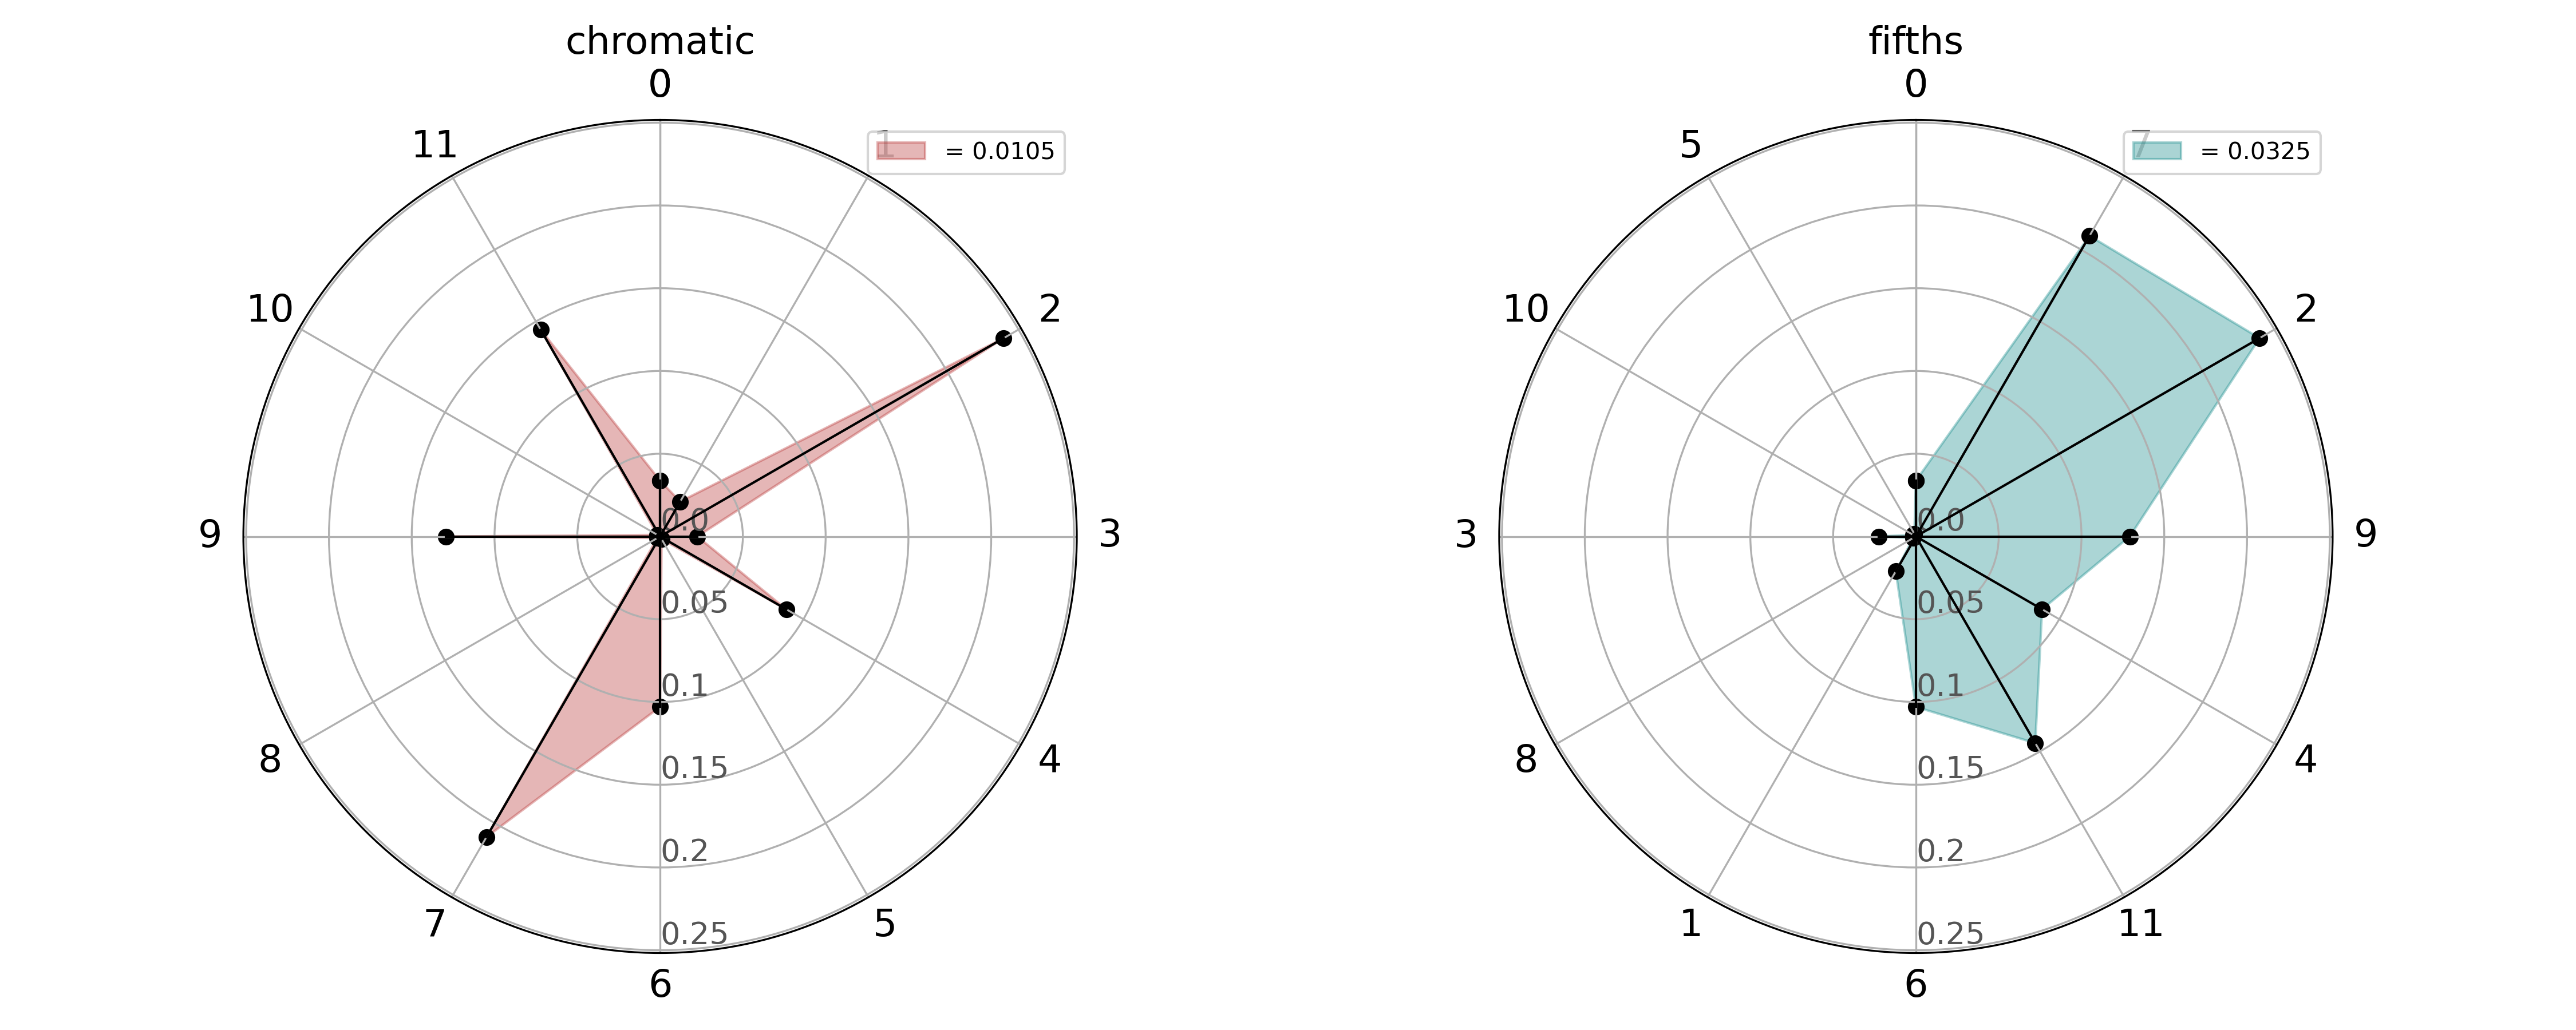
\includegraphics[width=\linewidth]{img/gesualdo.png}
    \caption{Gesualdo}
    \label{fig:gesualdo}
\end{figure}

\blindtext

\subsubsection{Lasso}

\blindtext

\begin{figure}[htbp]
    \centering
    
\includegraphics[width=\linewidth]{img/lasso.png}
    \caption{Lasso}
    \label{fig:lasso}
\end{figure}

\blindtext

\subsection{Diatonicism results in asymmetrical pitch-class distributions}

\textit{Instead of great composers, compare major vs minor? OR, rather: focus on the diatonicism vs chromaticism angle (see also~\cite{Cohn:2012}). Point is that there is a high correlation between historical period and "syntax", but there are exceptions (Gesualdo, Debussy)}

\subsubsection{Debussy}

\blindtext

\begin{figure}[htbp]
    \centering
    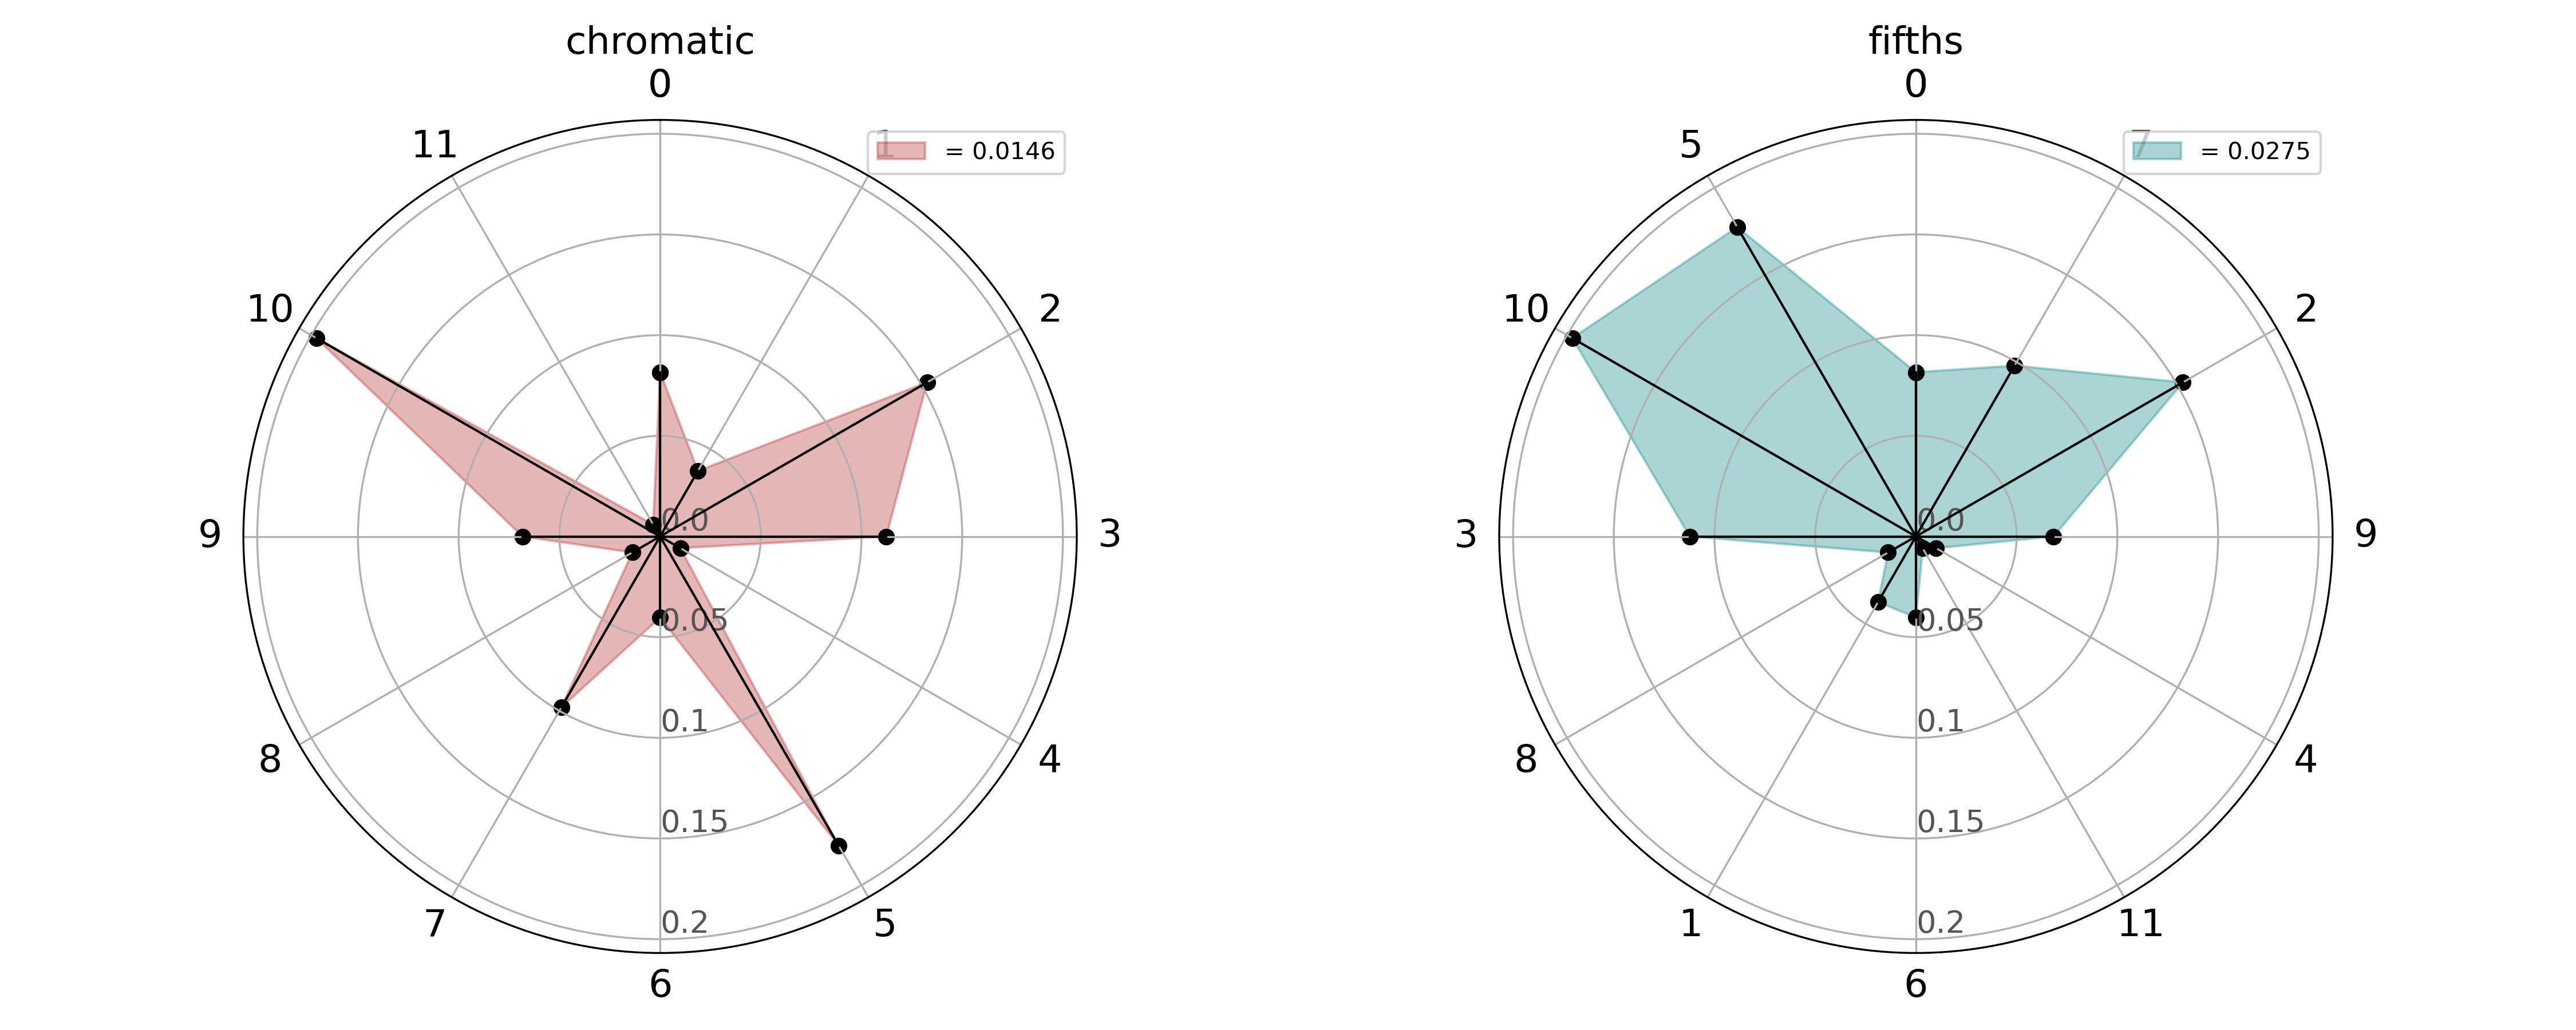
\includegraphics[width=\linewidth]{img/debussy.png}
    \caption{Debussy}
    \label{fig:debussy}
\end{figure}

\blindtext

\subsubsection{Bach}

\blindtext

\begin{figure}[htbp]
    \centering
    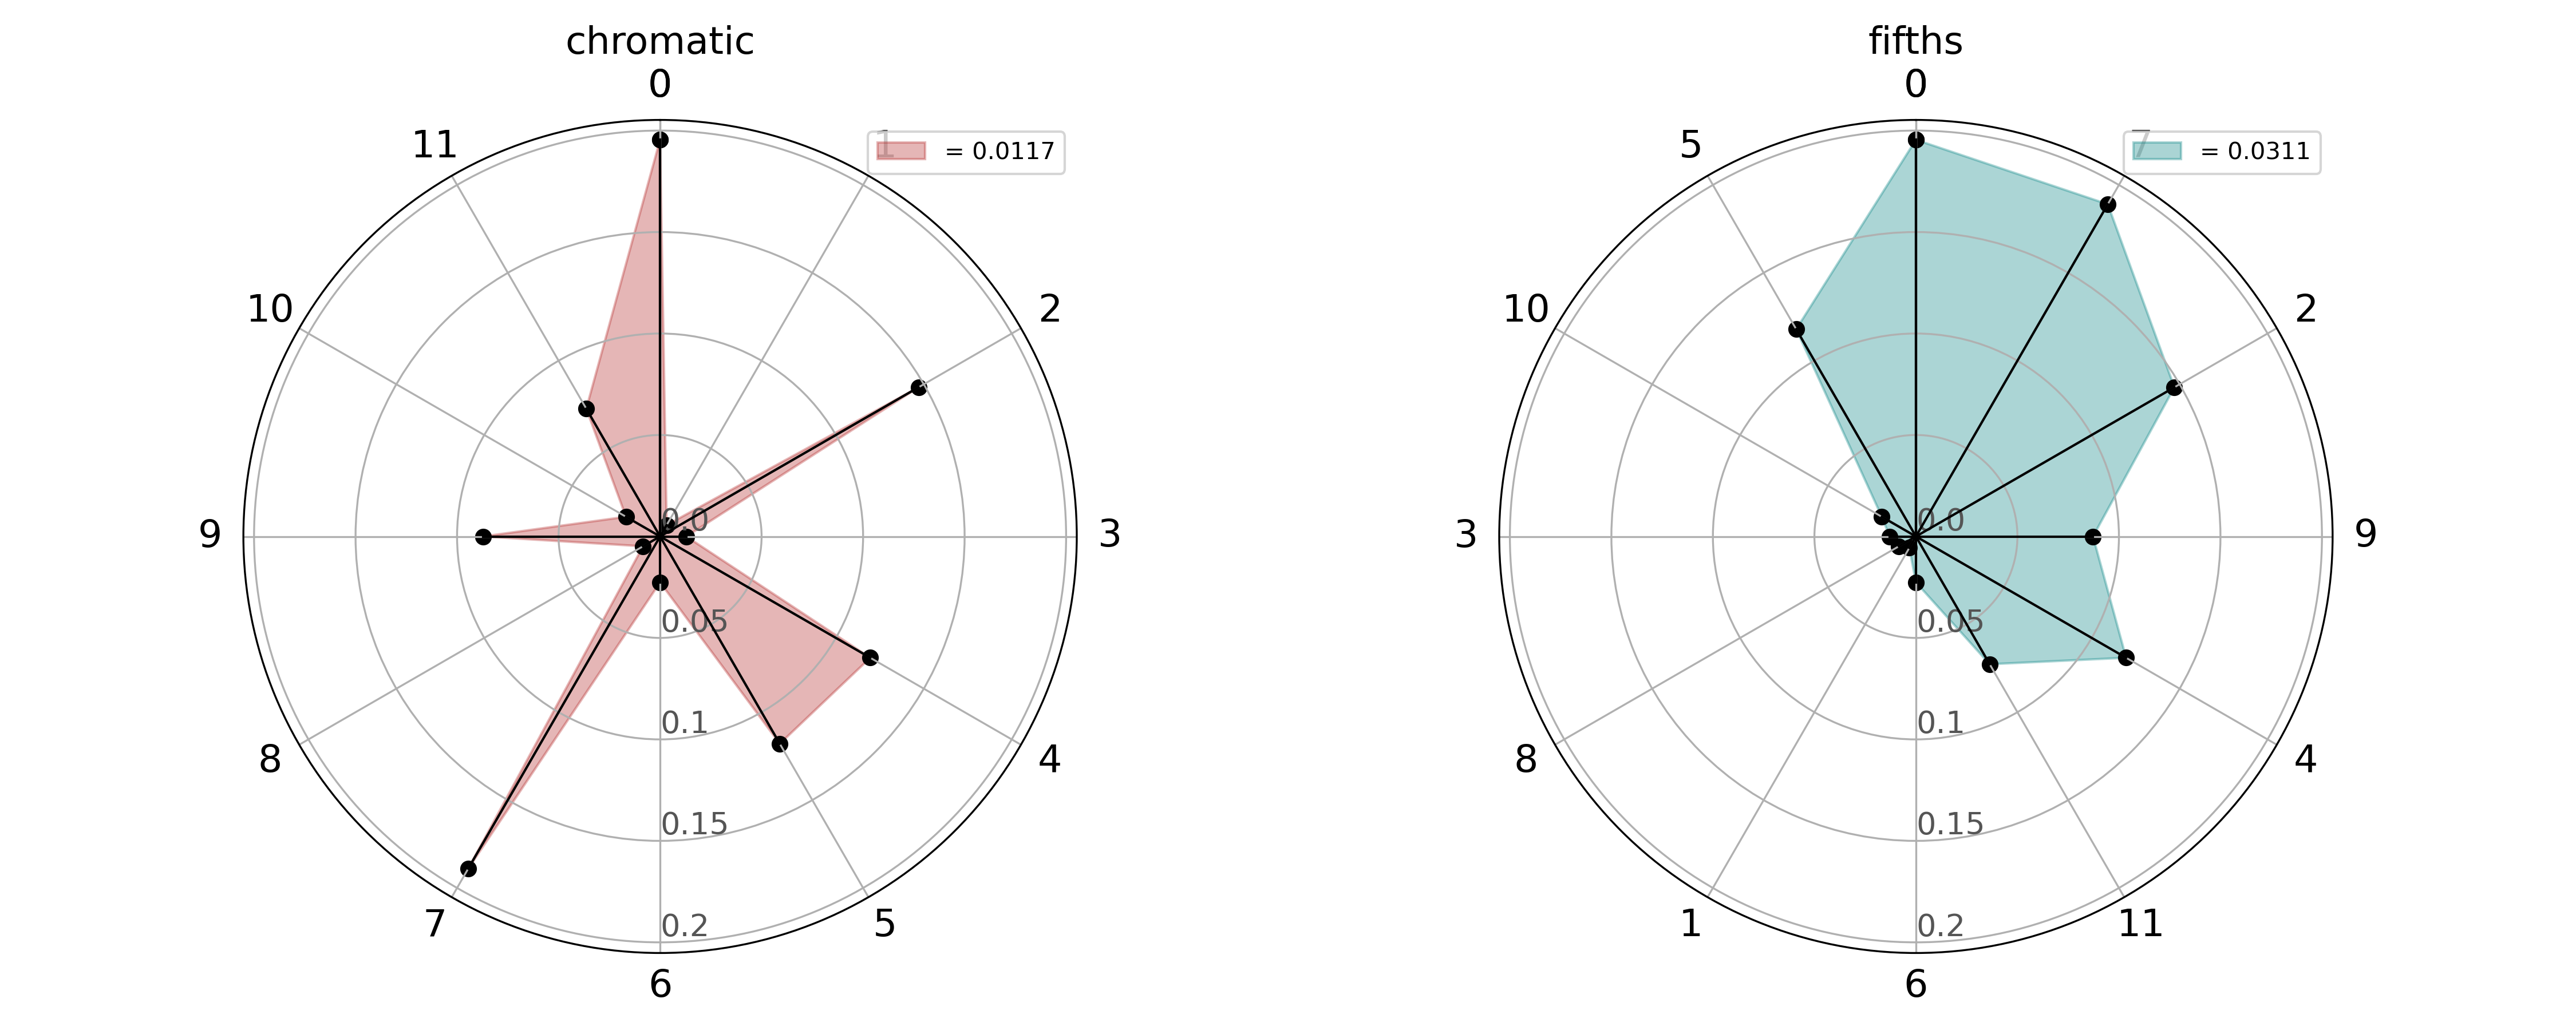
\includegraphics[width=\linewidth]{img/bach.png}
    \caption{Bach}
    \label{fig:bach}
\end{figure}

\blindtext


\subsubsection{Mozart}

\blindtext

\begin{figure}[htbp]
    \centering
    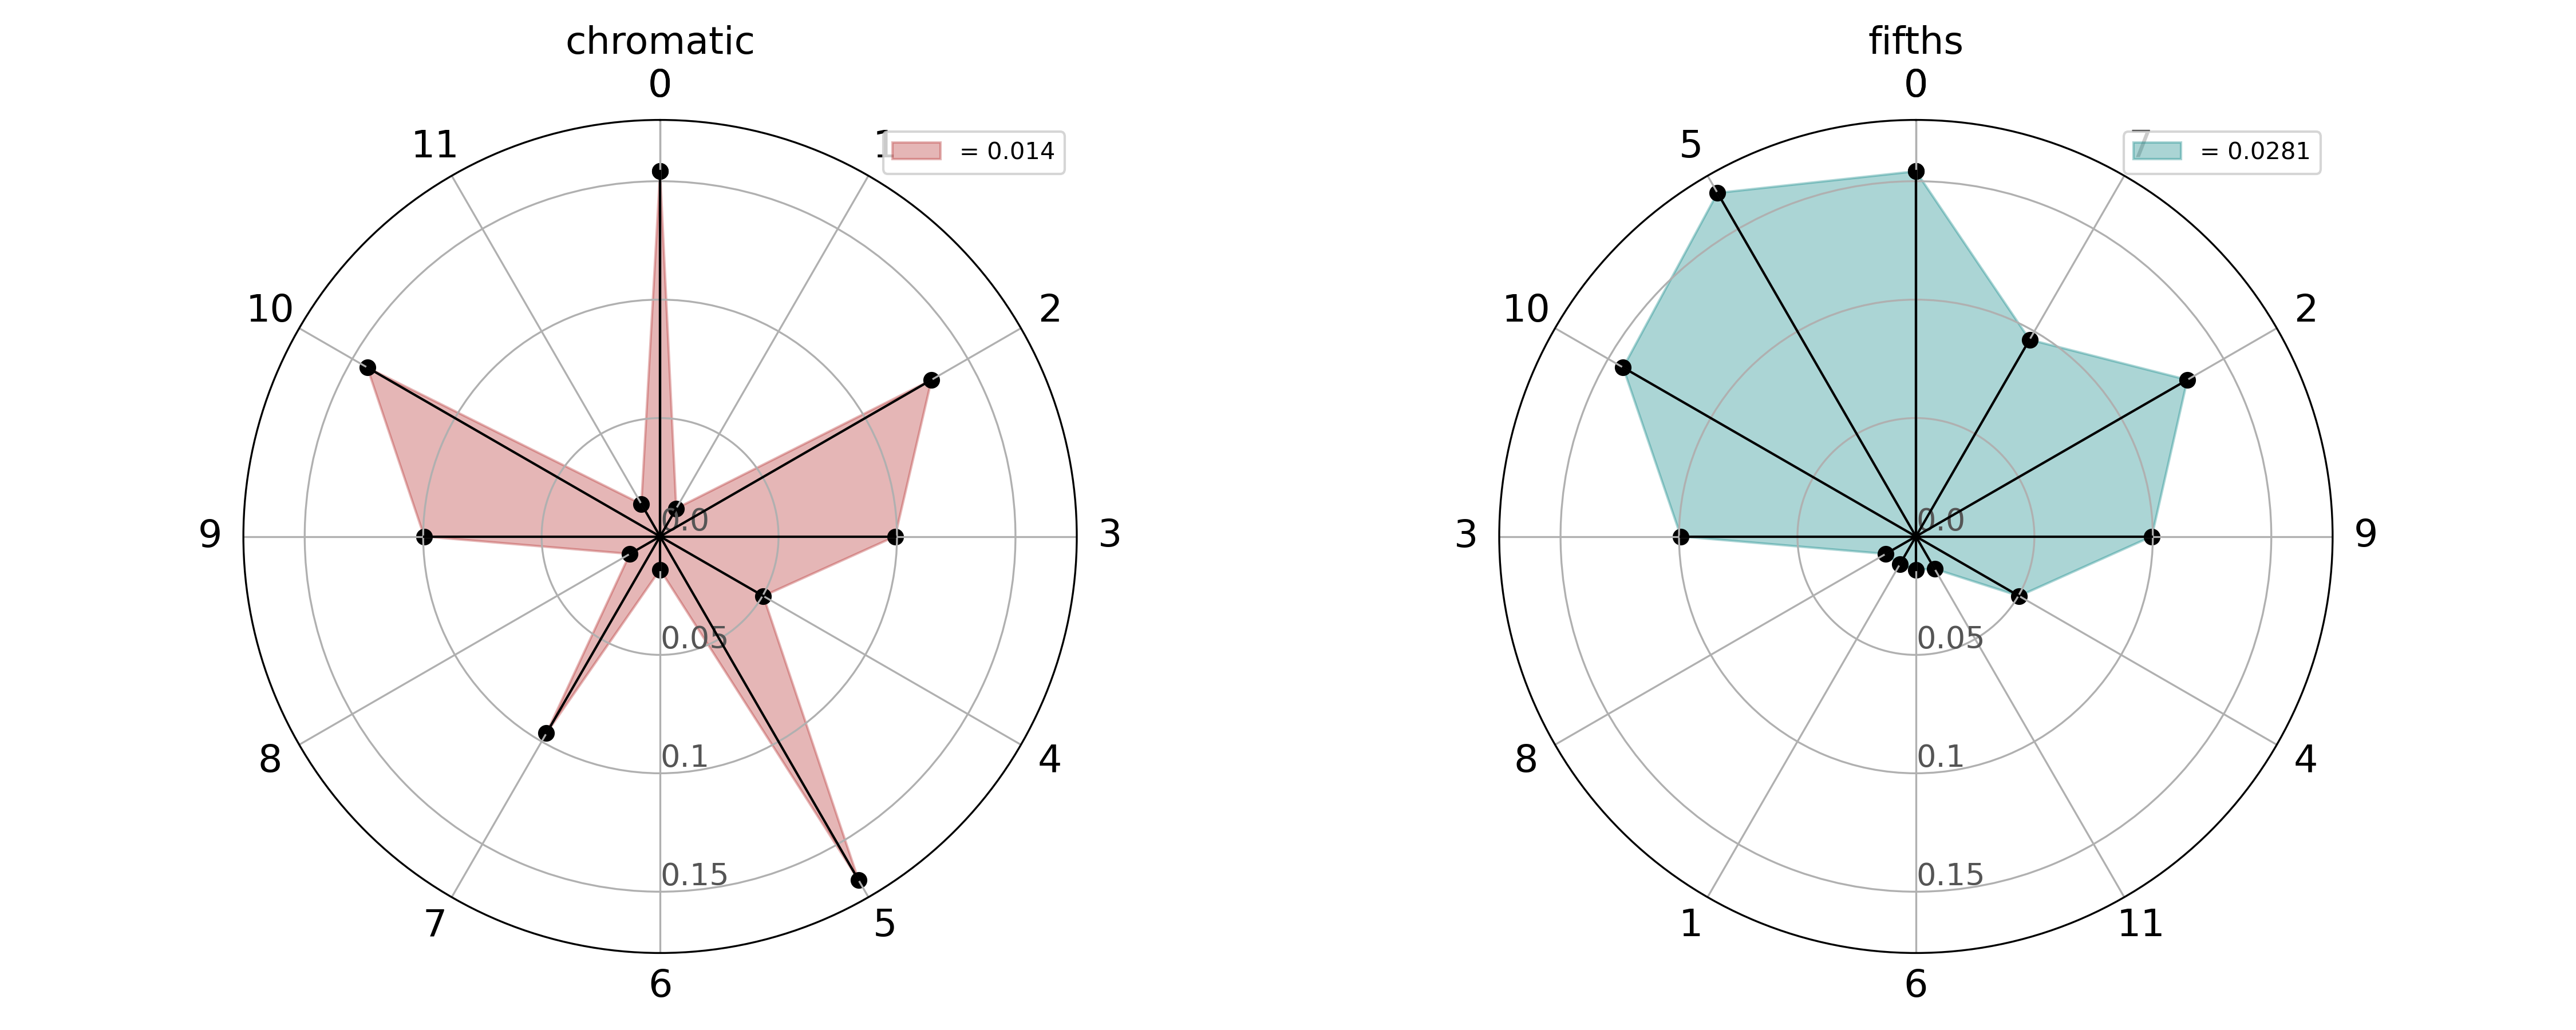
\includegraphics[width=\linewidth]{img/mozart.png}
    \caption{Mozart}
    \label{fig:mozart}
\end{figure}

\blindtext

\subsubsection{Beethoven}

\blindtext

\begin{figure}[htbp]
    \centering
    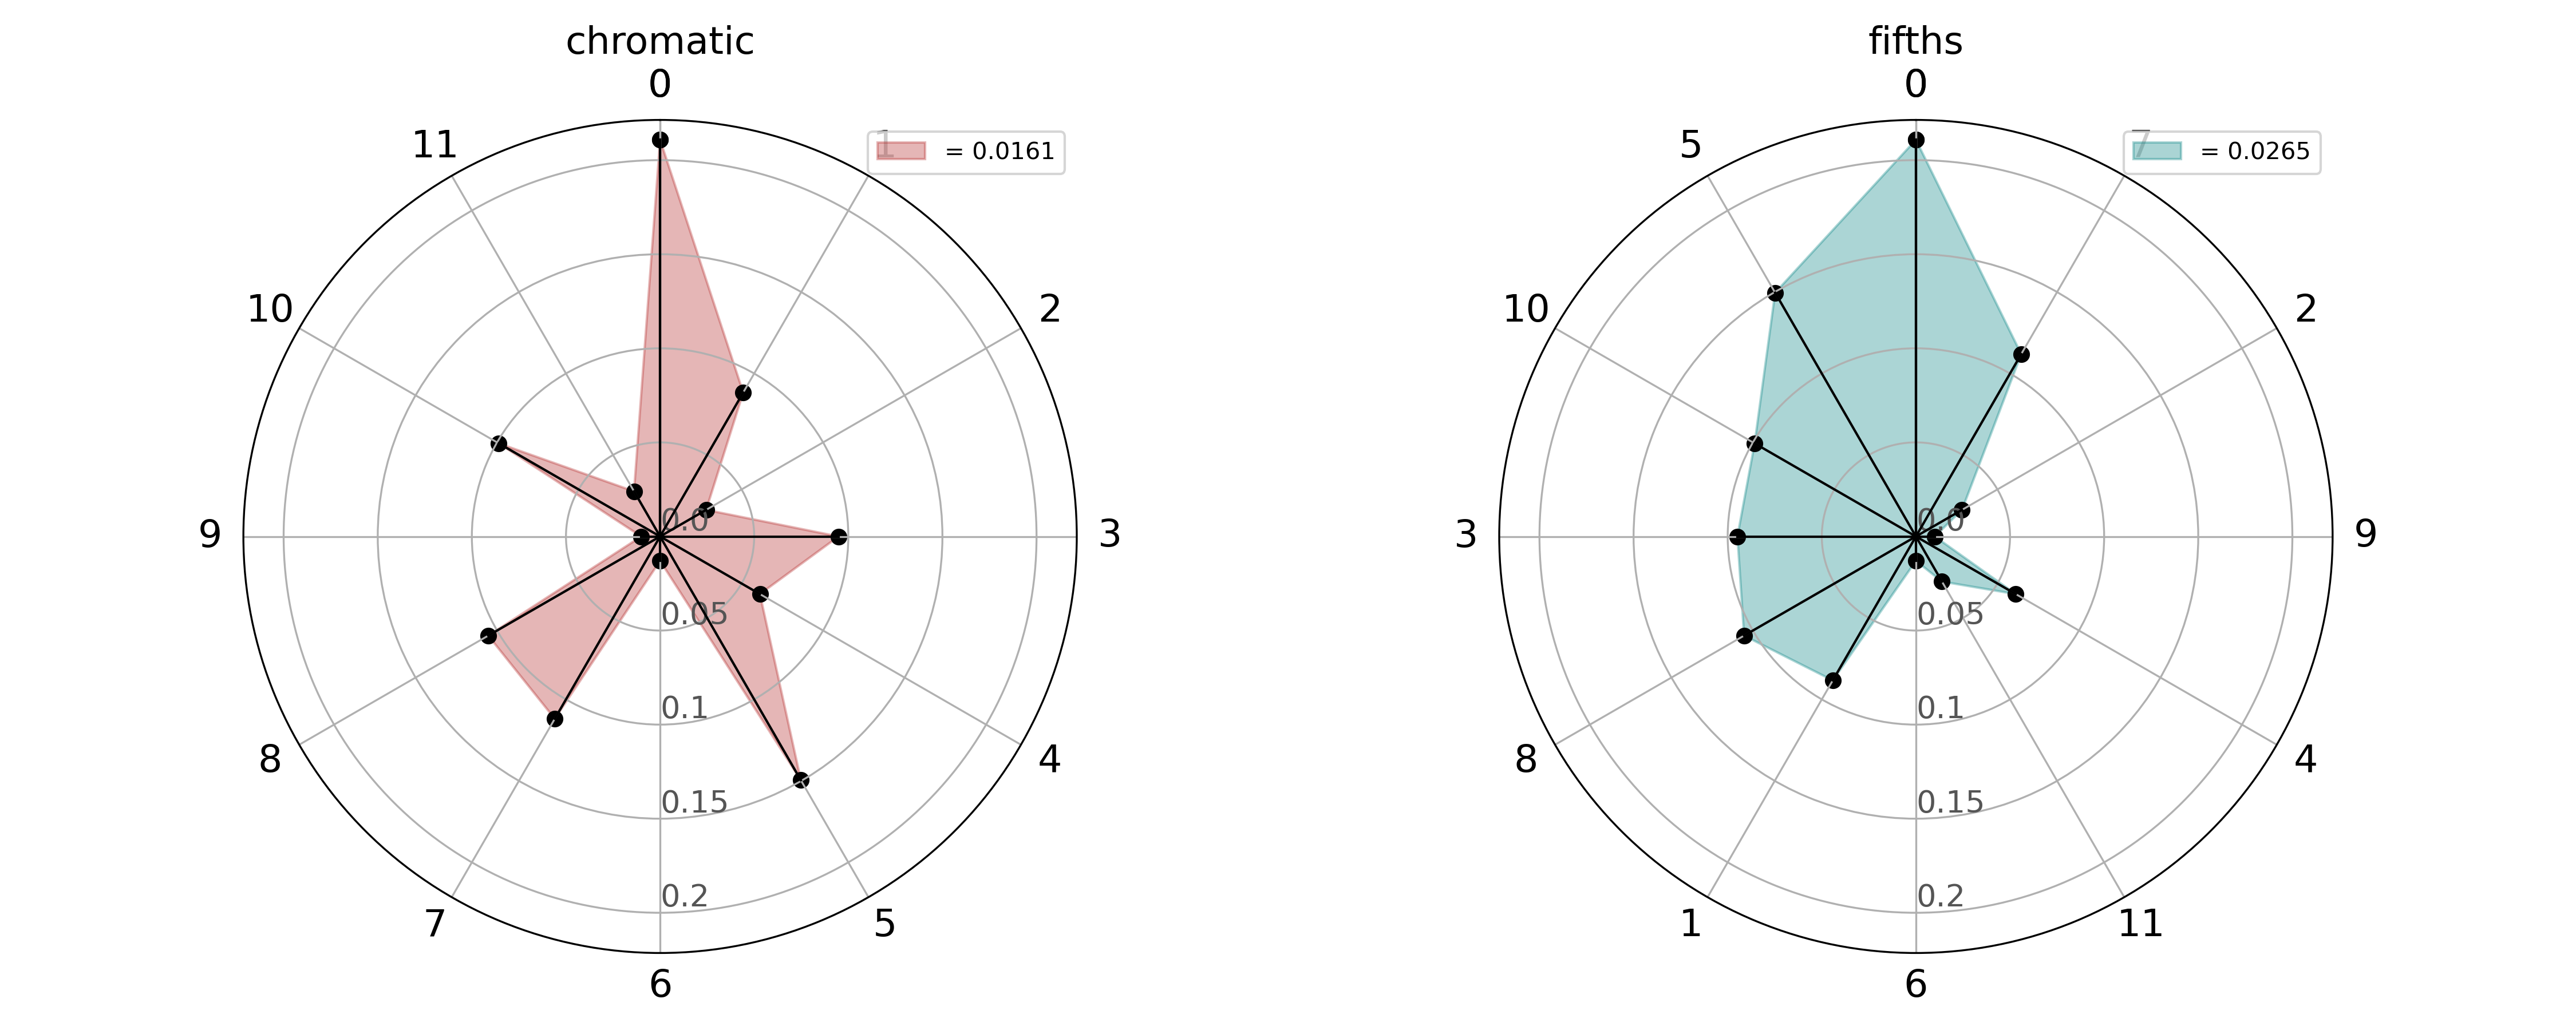
\includegraphics[width=\linewidth]{img/beethoven.png}
    \caption{Beethoven}
    \label{fig:beethoven}
\end{figure}

\blindtext

\subsubsection{Schubert}

\blindtext

\begin{figure}[htbp]
    \centering
    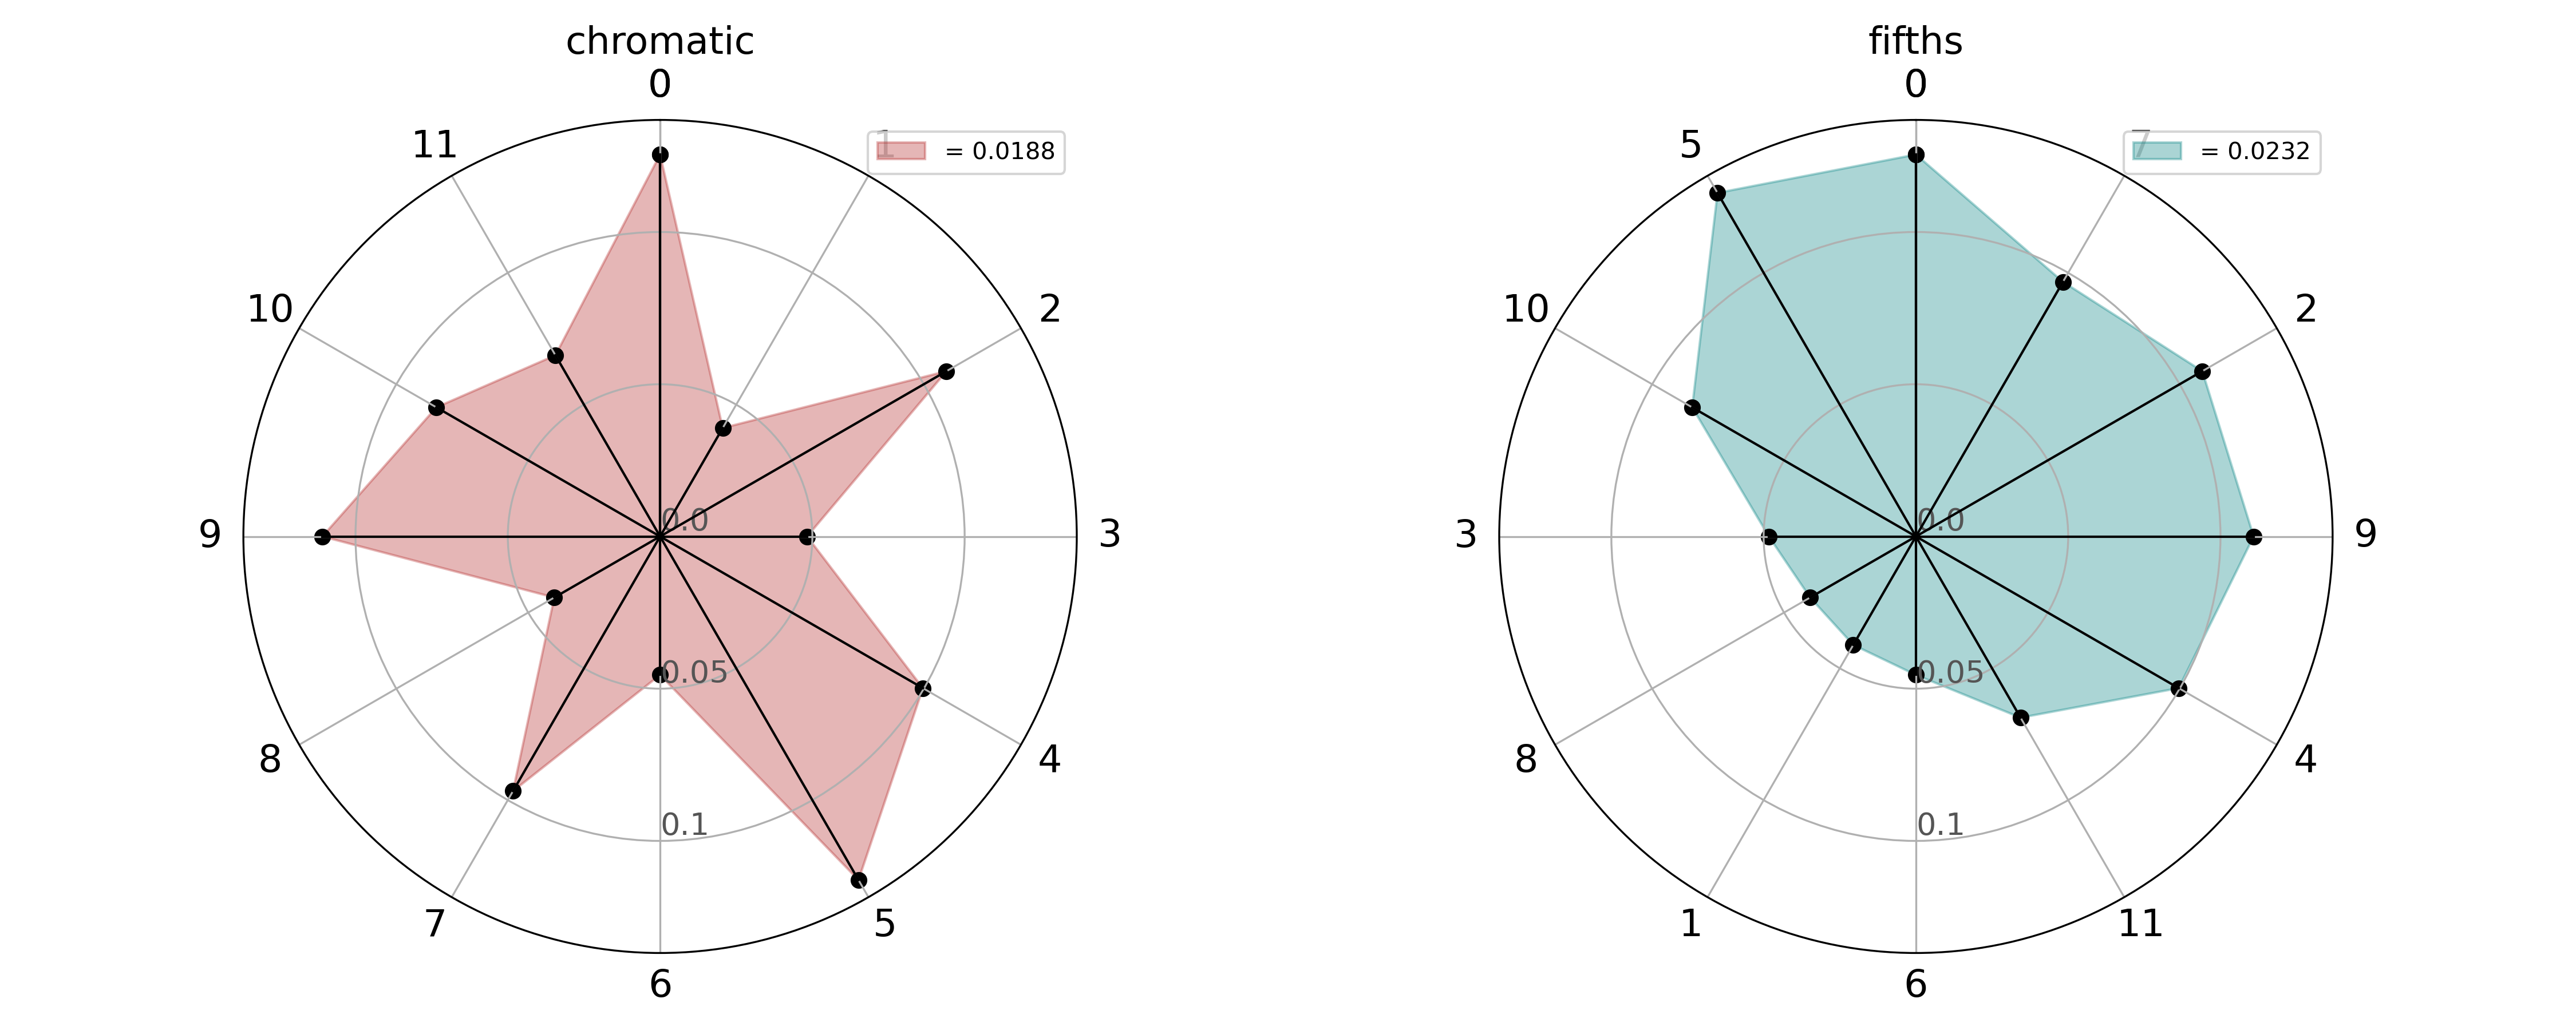
\includegraphics[width=\linewidth]{img/schubert.png}
    \caption{Schubert}
    \label{fig:schubert}
\end{figure}

\blindtext

\subsubsection{Hensel}

\blindtext

\begin{figure}[htbp]
    \centering
    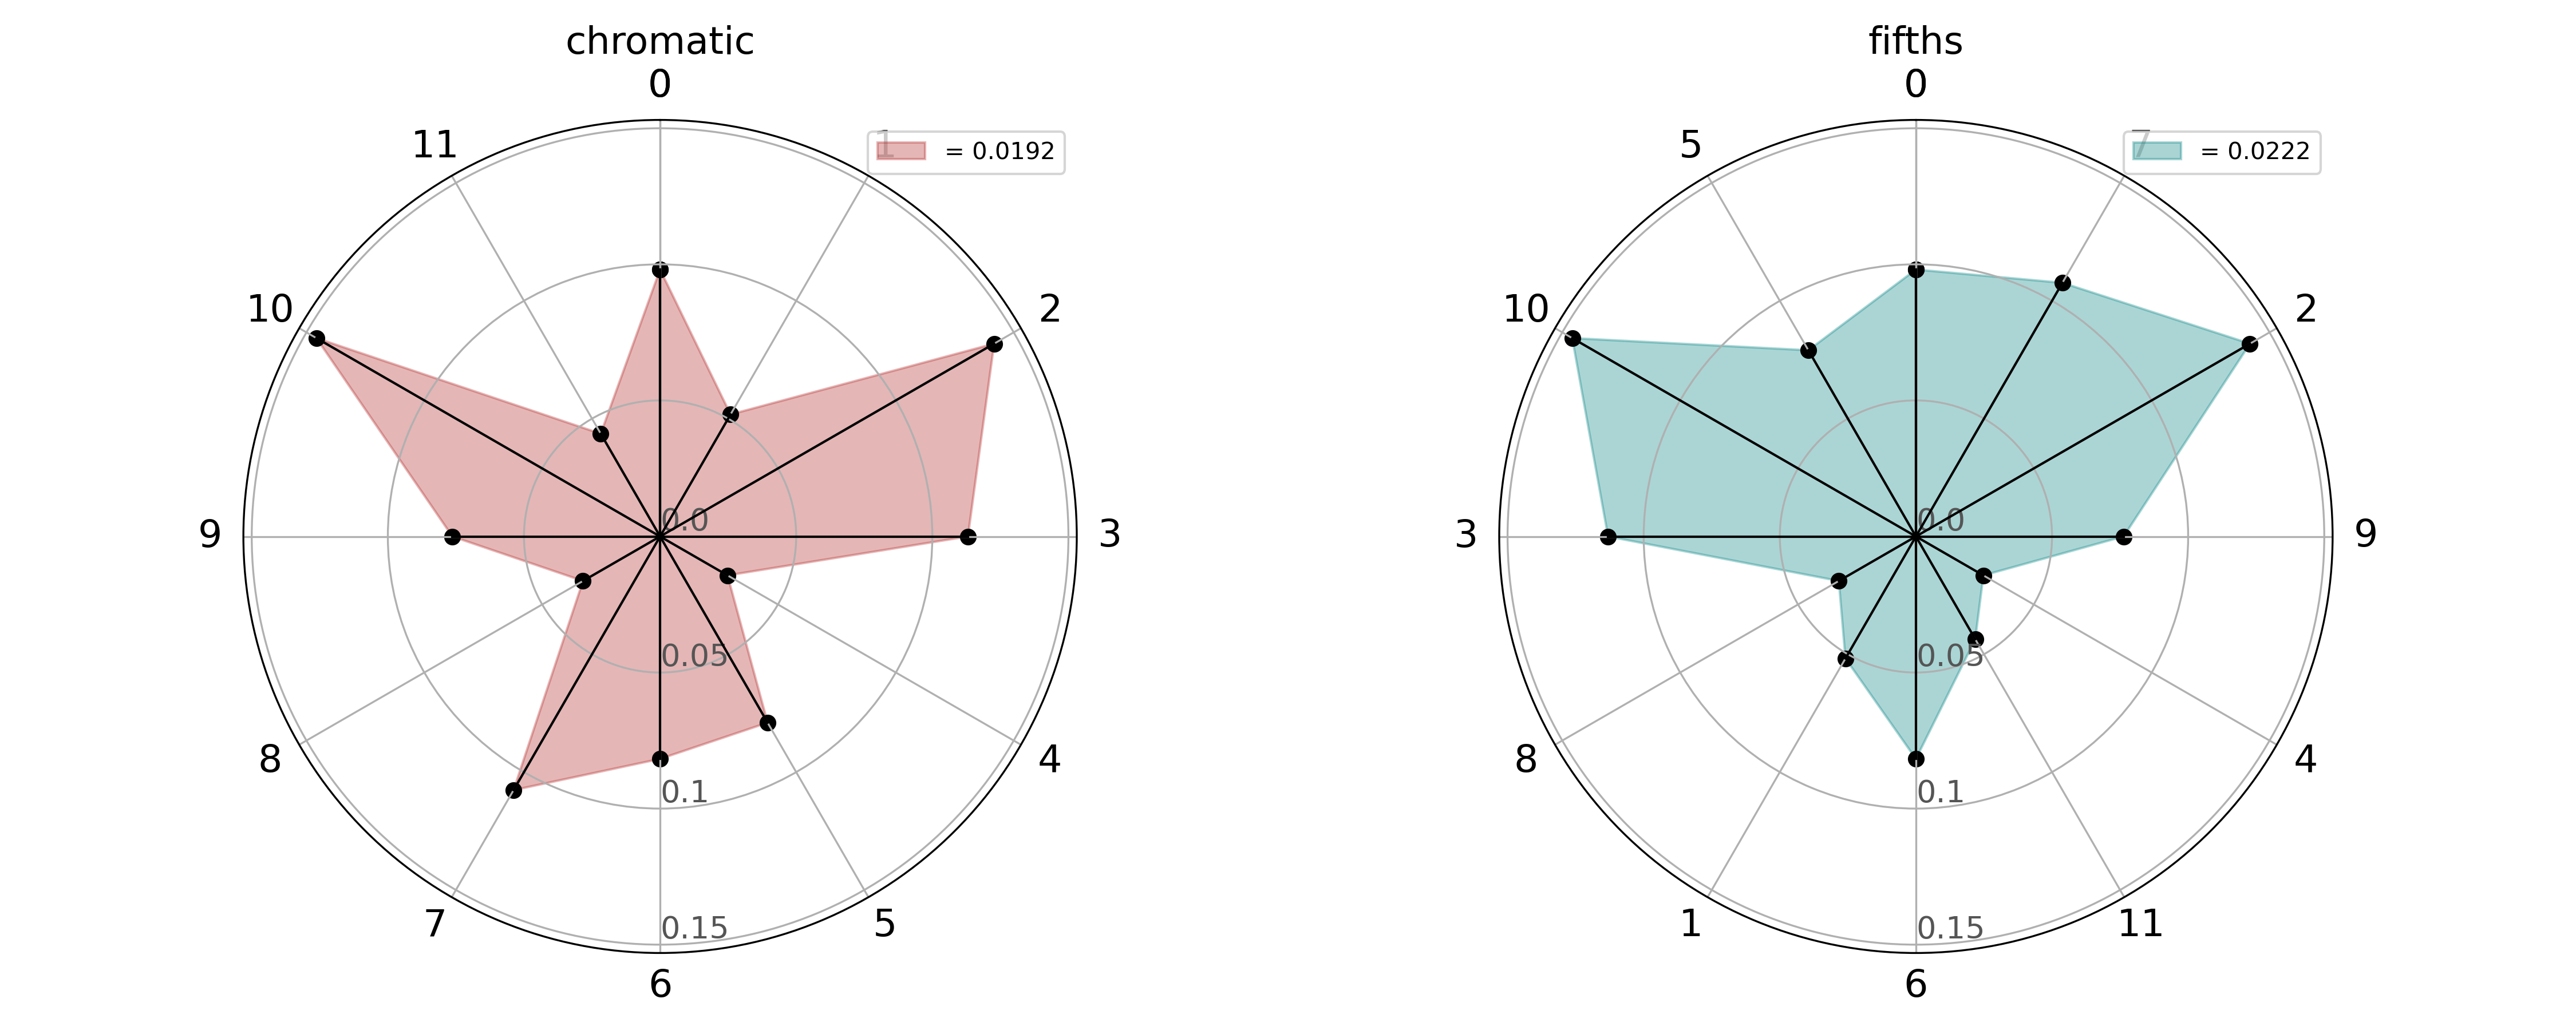
\includegraphics[width=\linewidth]{img/hensel.png}
    \caption{Hensel}
    \label{fig:hensel}
\end{figure}

\blindtext

\subsection{Chromaticism features nearly-symmetrical pitch-class distributions}

\subsubsection{Liszt}

\blindtext

\begin{figure}[htbp]
    \centering
    
\includegraphics[width=\linewidth]{img/liszt.png}
    \caption{Webern}
    \label{fig:liszt}
\end{figure}

\subsubsection{Scriabin}

\blindtext

\begin{figure}[htbp]
    \centering
    
\includegraphics[width=\linewidth]{img/scriabin.png}
    \caption{Scriabin}
    \label{fig:scriabin}
\end{figure}

\blindtext

\subsubsection{Mahler}

\blindtext

\begin{figure}[htbp]
    \centering
    
\includegraphics[width=\linewidth]{img/mahler.png}
    \caption{Mahler}
    \label{fig:mahler}
\end{figure}

\blindtext

\subsubsection{Vaughan-Williams}

\blindtext

\begin{figure}[htbp]
    \centering
    
\includegraphics[width=\linewidth]{img/vaughan_williams.png}
    \caption{Vaughan-Williams}
    \label{fig:vaughan_williams}
\end{figure}

\blindtext

\subsubsection{Webern}

\blindtext % Dummy text

\begin{figure}[htbp]
    \centering
    
\includegraphics[width=\linewidth]{img/webern.png}
    \caption{Webern}
    \label{fig:webern}
\end{figure}

\begin{itemize}
\item Donec dolor arcu, rutrum id molestie in, viverra sed diam
\item Curabitur feugiat
\item turpis sed auctor facilisis
\item arcu eros accumsan lorem, at posuere mi diam sit amet tortor
\item Fusce fermentum, mi sit amet euismod rutrum
\item sem lorem molestie diam, iaculis aliquet sapien tortor non nisi
\item Pellentesque bibendum pretium aliquet
\end{itemize}

See example in Table ~\ref{tab1}.
%------------------------------------------------

\section{Hierarchical analysis}

Wavescapes, pitchscapes, samples to StarPlots

\blindtext

\section{Diachronic analyses}

\subsection{Diatonicism vs Chromaticism}

\subsection{Comparing different styles and genres}

\blindtext

\textbf{Important: add also composers' names that do \textit{not} fit the narrative. Discuss here briefly, and in more detail in the general discussions that example-based music historiography and style analysis is prone to confirmation bias regarding a linear, progressive version of music (``evolution'' in the wrong sense). It is particularly important to also regard conflicting examples. It is crucial to determine whether those are `outliers', or whether they refute one's theory of style evolution.}

\begin{figure}
    \centering
    
\includegraphics[width=\linewidth]{img/diatonicismVsChromaticism.png}
    \caption{Diatonicism vs Chromaticism}
    \label{fig:diavschr}
\end{figure}

\blindtext

\subsubsection{Western classical music}

\blindtext

\begin{figure}
    \centering
    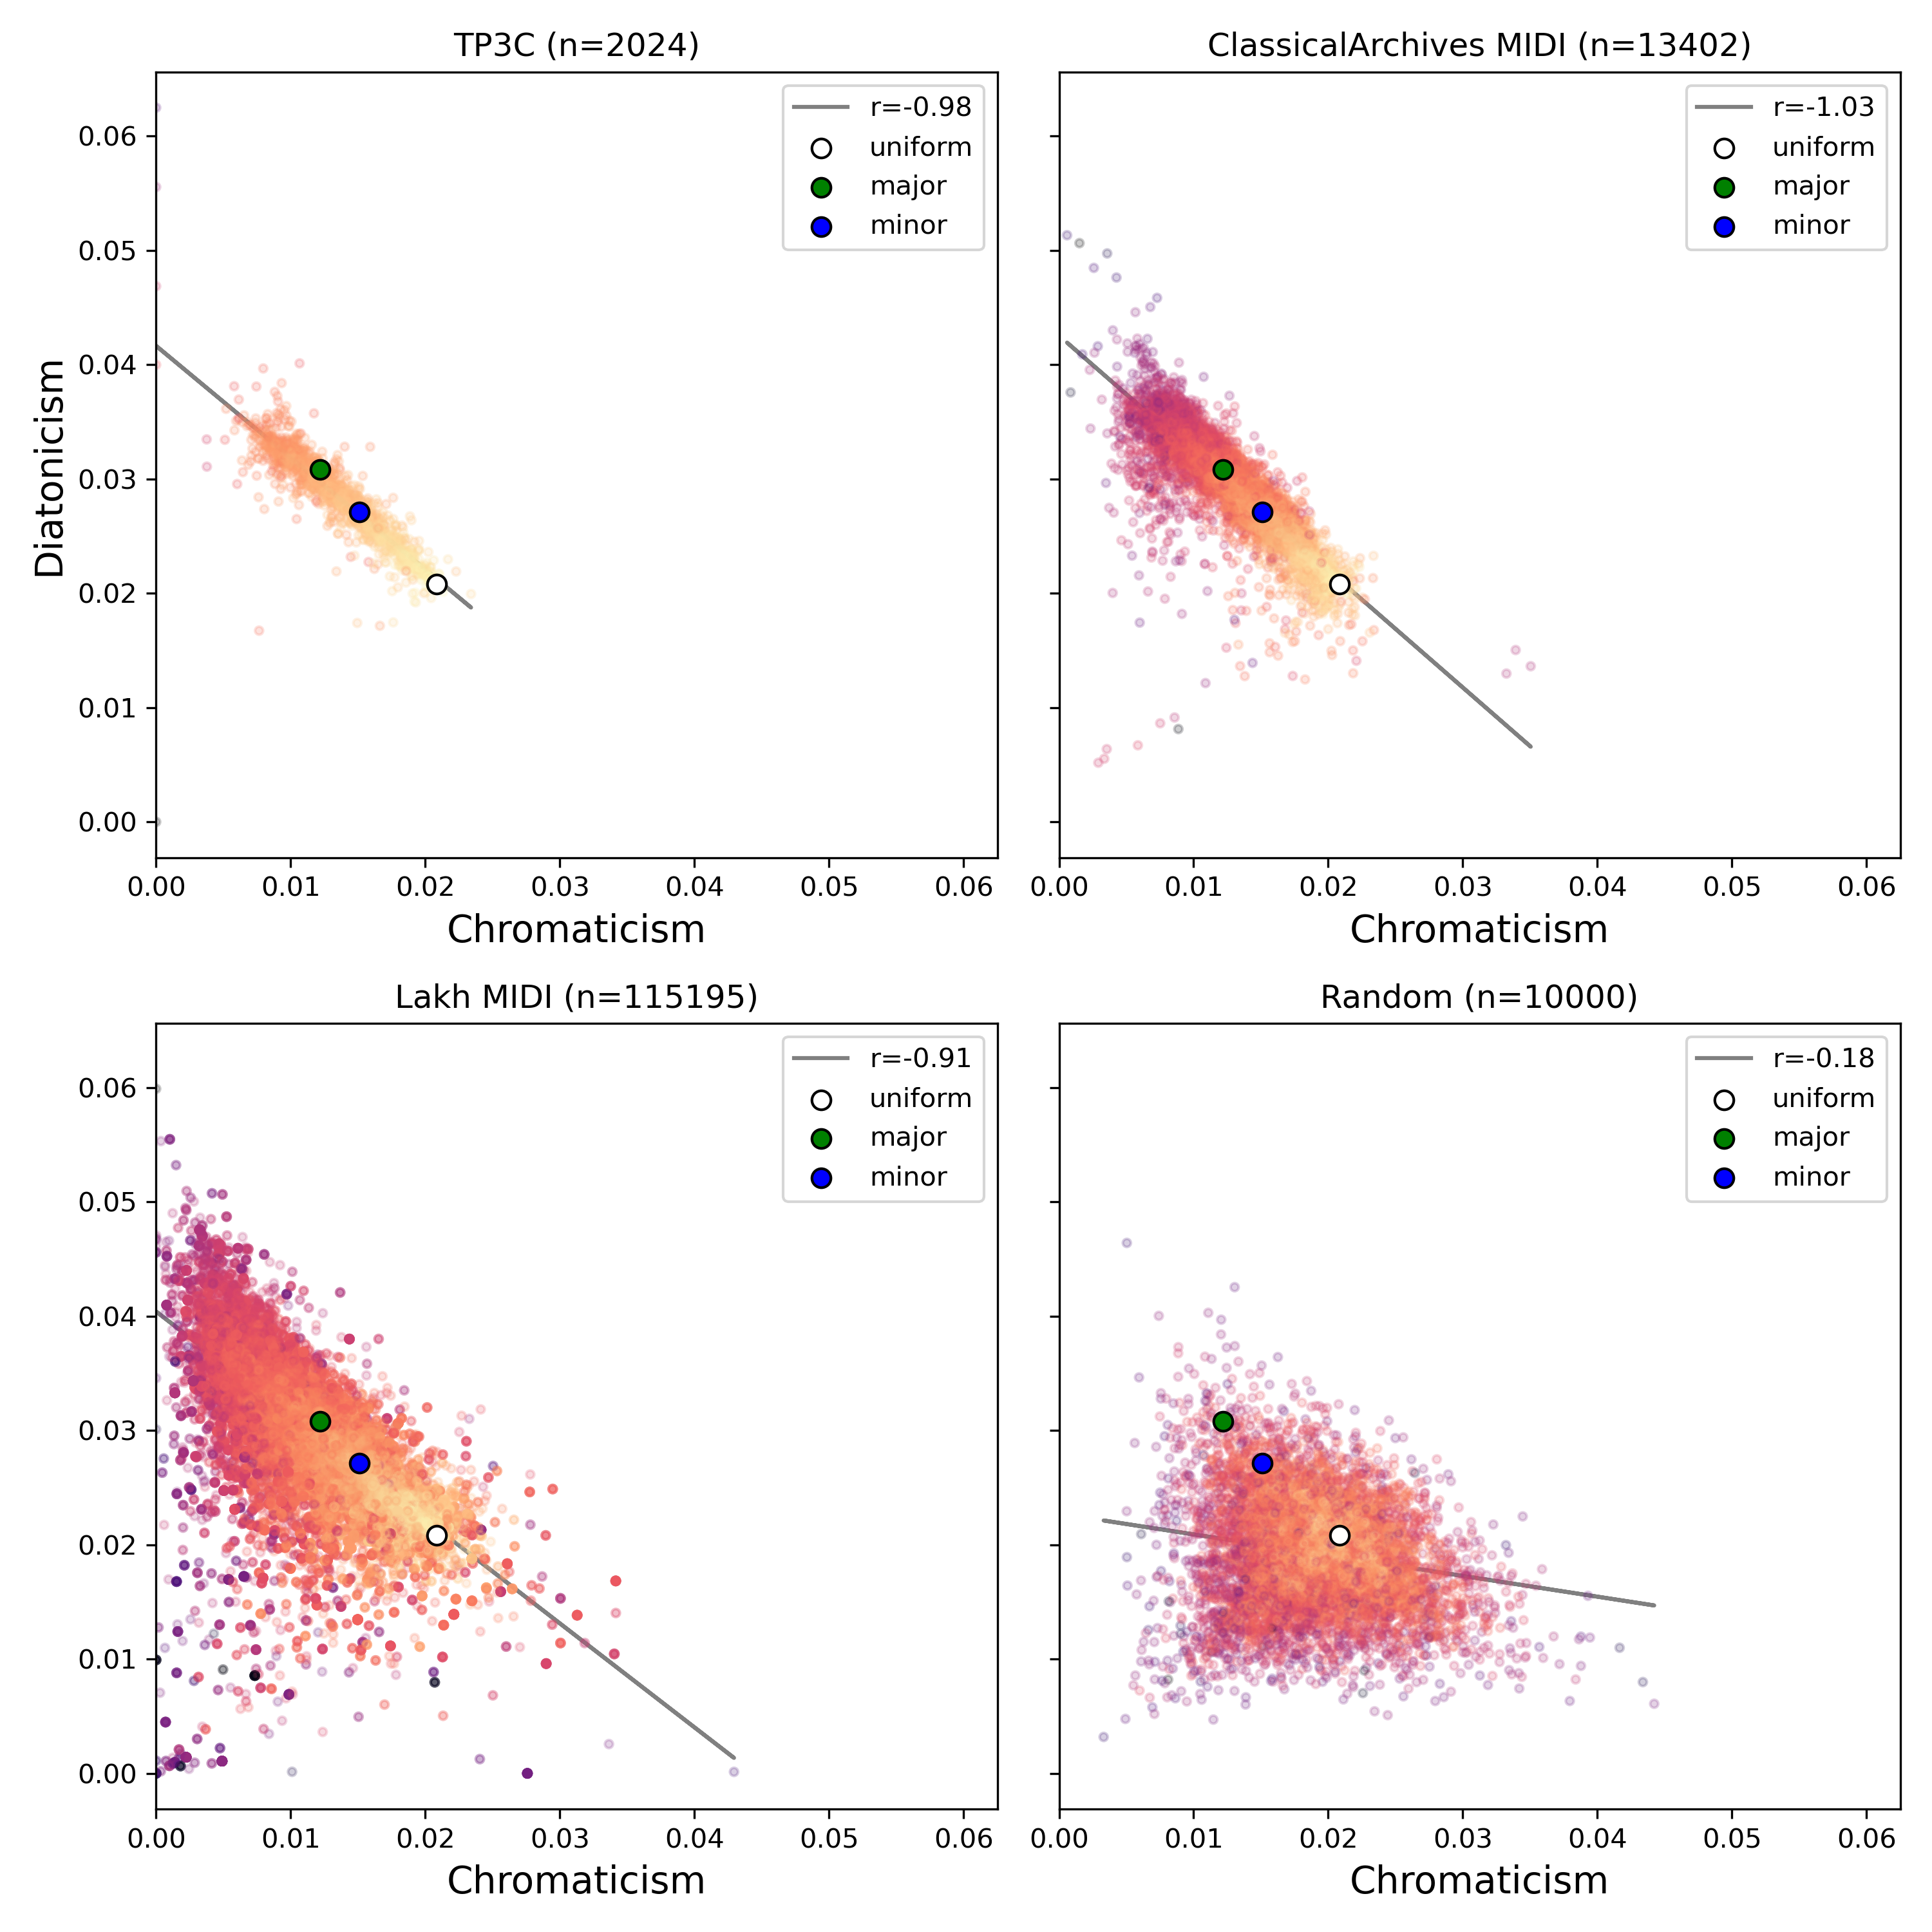
\includegraphics[width=\linewidth]{img/comparison_datasets.png}
    \caption{Comparison of large-scale behavior in different datasets. }
    \label{fig:historical_dists}
\end{figure}

\subsubsection{Pop/Rock}

\blindtext

\section{General discussion \& Conclusions}

\blindtext % Dummy text

\begin{equation}
\label{eq:emc}
e = mc^2
\end{equation}

\blindtext % Dummy text

%----------------------------------------------------------------------------------------
%	REFERENCE LIST
%----------------------------------------------------------------------------------------

\begin{thebibliography}{99} % Bibliography - this is intentionally simple in this template

\bibitem{Figueredo:2009}
Figueiredo, A. J., and Wolf, P. S. A. 2009.
\newblock Assortative pairing and life history strategy - a cross-cultural
  study.
\newblock \textit {Human Nature}, vol. 20, pp. 317--330.

\bibitem{Berry:1976}
Berry, W. 1976.
\newblock \textit {Structural Functions in Music}.
\newblock New England: Dover.

\bibitem{Cohn:2012}
Cohn, R. 2012. 
\newblock \textit{Audacious Euphony: Chromatic Harmony and the Triad's Second Nature}. 
\newblock Oxford: Oxford University Press.

\bibitem{tp3c}
Moss, F. C., Neuwirth, M., and Rohrmeier, M. 2020. \textit{Tonal Pitch-Class Counts Corpus (TP3C)}. Zenodo. \url{https://doi.org/10.5281/zenodo.3600088}.

\bibitem{YustAmiot:2022}
Yust, J. and Amiot, E. 2022. 
\newblock \textit {Non-spectral Transposition-Invariant Information in Pitch-Class Sets and Distributions}
\newblock In \textit{Mathematics and Computation in Music}, ed. by M. Montiel, O. A. Agustín-Aquino, F. Gómez, J. Kastine, E. Lluis-Puebla, and B. Milam, 279--91. Lecture Notes in Computer Science. Cham: Springer International Publishing. \url{https://doi.org/10.1007/978-3-031-07015-0_23}.


 
\end{thebibliography}

\noindent For more information \url{http://www.chicagomanualofstyle.org/tools_citationguide.html}

%----------------------------------------------------------------------------------------

\end{document}
